
\documentclass[journal,onecolumn]{IEEEtran}
\usepackage{cite}
\usepackage{url}
\usepackage{booktabs}
\usepackage{longtable}
\usepackage{array}
\usepackage{enumitem}
\usepackage{tikz}
\usetikzlibrary{arrows.meta,positioning,shapes.geometric,fit,calc}
\usepackage{balance}
\usepackage{graphicx}
\usepackage{amsmath}
\setlist[itemize]{leftmargin=*,nosep}
\setlist[enumerate]{leftmargin=*,nosep}
\title{JPCM-1.0 and the Joint Master Control Plane: A Critique-Hardened Protocol, Authority Kernel, and Attention Firewall for Autonomous Engineering Systems}
\author{Jepson Taylor\\Veox AI\\\texttt{jepson@veox.ai}}
\begin{document}
\maketitle
\begin{abstract}
Autonomous software agents are becoming capable enough to perform useful engineering work, but their surrounding control systems are not yet rigorous enough to trust. Tool protocols expose capabilities; agent protocols coordinate workers; dashboards show activity; coding agents modify repositories. None of these, by themselves, provides a sovereign authority layer that can decide what may happen, what must be proven, what the user must see, and what the system should learn. This paper specifies the Joint Master Control Plane (JMCP) and its mandatory communication protocol, Joint Process Control Messaging version 1.0.0 (JPCM-1.0). JMCP is defined as an authority, evidence, attention, and process-control plane for autonomous engineering systems. JPCM-1.0 is a versioned, signed, replayable, policy-bound protocol used by all services, agents, adapters, tools, data sources, voice surfaces, and user interfaces. We conduct a hostile review of the prior V5 artifact bundle, score each artifact using a 100-point engineering rubric, and convert the criticisms into normative protocol and architecture requirements. The resulting design includes capability leases, typed work orders, task DAGs, evidence bundles, attention packets, voice-confirmation semantics, tool and data registries, self-improvement governance, automated tool-building workflows, and conformance levels. The central claim is that useful autonomy is not achieved by adding more agents. It is achieved by increasing agency only when evidence quality, containment, observability, and user-attention quality improve faster than autonomy.
\end{abstract}
\begin{IEEEkeywords}
AI agents, control plane, protocol design, autonomous software engineering, observability, evidence, tool security, prompt injection, voice interfaces, self-improvement, JPCM, JMCP.
\end{IEEEkeywords}

\section{Introduction}
Autonomous engineering systems now combine language models, tool routers, sandboxes, repositories, continuous integration, issue trackers, documentation, web search, data stores, and communication channels. The operational problem is no longer simply whether a model can produce a patch. The deeper problem is whether an authority layer can decide what work should be attempted, which agent may attempt it, what data it may see, what tools it may call, what evidence proves completion, what should be learned, what should be forgotten, and when the human should be interrupted. A model that writes code is not a control plane. A dashboard that shows logs is not an authority. A protocol that exposes tools is not a safety model.

The Joint Master Control Plane (JMCP) is proposed as the missing supervisory layer. It is inspired by industrial process control and fault detection, but applied to agentic engineering. Like a semiconductor fab control system, it must observe many concurrent activities, detect anomalies, manage bottlenecks, preserve yield, route work, suppress noise, escalate only important decisions, and continuously improve the process. Unlike a factory controller, it must also handle natural language, voice, untrusted code, untrusted web content, malicious tool descriptions, software supply chains, model hallucination, prompt injection, memory poisoning, and self-improving agents.

The accompanying protocol, JPCM-1.0, is the central contribution. It defines how every program talks to JMCP and how JMCP talks back. It is not merely an event envelope. It is a standard object model for work orders, tasks, leases, workflows, evidence, tools, data assets, memory proposals, self-improvement proposals, attention packets, voice segments, policy decisions, telemetry, and conformance. This matters because informal control-plane prose is not enough. If every service reports ``task complete'' differently, if tools make side effects without leases, if evidence is not replayable, or if voice commands bypass risk gates, the system collapses into a dashboard over inconsistent lies.

\section{Contributions}
This paper makes six contributions. First, it defines JMCP by both positive and negative boundaries: what it is and what it is not. Second, it presents a hostile review and scorecard for the uploaded V5 corpus. Third, it specifies JPCM-1.0 as a normative control protocol. Fourth, it introduces an attention firewall for minimum-safe user interruption across text and voice. Fifth, it specifies tool/data/model awareness and an automated tool-building loop. Sixth, it defines a self-improvement process that allows the system to improve without letting the judged component rewrite the judge.

\section{Hostile Review and Scorecard}
The V5 bundle contains four engineering specifications, four paper drafts, one scorecard, and two schema drafts. The best documents already reject common category errors: JMCP is not a chatbot, not a CI wrapper, not an MCP server, and not an agent framework. They correctly emphasize authority, evidence, leases, attention, and protocol. The remaining weakness is operational finality. The protocol is described, but the schema is still too narrow. The most important missing pieces are complete payload definitions, self-improvement semantics, automated tool-building tasks, voice-confirmation rules, conformance classes, and semantic constraints that are not expressible in JSON Schema alone.

\begin{table*}[t]
\centering
\caption{V5 artifact scores under the final critique rubric. Scores measure buildability and defensibility, not prose polish.}
\scriptsize
\begin{tabular}{p{0.34\textwidth}p{0.06\textwidth}p{0.52\textwidth}}
\toprule
Artifact & Score & Critical feedback\\
\midrule
JMCP\_V4\_ENGINEERING\_SPEC.md & 87 & Still too permissive around schema extensions, lacks exhaustive payload definitions, and doe\\
JMCP\_V4\_engineering\_spec(1).md & 89 & Needs a harder conformance story, adapter certification, and mandatory message semantics for\\
jmcp\_v4\_protocol\_first\_engineering\_spec.md & 92 & Needs a complete schema, explicit task-kind universe, semantic constraints not expressible i\\
jmcp\_v4\_protocol\_first\_engineering\_spec(1).md & 90 & Less complete than the main protocol-first spec; weaker scorecard and thinner conformance/ev\\
JMCP\_V4\_ieee\_whitepaper.tex & 86 & Too short for a final reference paper; protocol is described but not made fully normative, a\\
jmcp\_v4\_ieee\_white\_paper.tex & 88 & Needs final schema alignment, more figures, deeper task semantics, and stronger claims about\\
jmcp\_v4\_protocol\_first\_ieee\_paper.tex & 91 & Still 10 pages rather than the requested final 20-30; references and diagrams are not enough\\
jmcp\_v4\_whitepaper.tex & 89 & Needs tighter normative language, more adversarial evaluation, final JSON schema mapping, an\\
jmcp\_v4\_scorecard.md & 82 & Not a buildable artifact; does not score the V5 bundle, and does not convert every criticism\\
jmcp\_cp\_v1\_envelope.schema.json & 71 & Too envelope-only. Missing service manifests, work orders, tasks, workflows, evidence bundle\\
jmcp\_v4\_jpcp\_v1\_envelope\_schema.json & 73 & Still under-specified as a protocol standard. It cannot validate the actual universe of JPCM\\
\bottomrule
\end{tabular}
\end{table*}

The scorecard yields a clear diagnosis. The architecture is strong; the standard is incomplete. A system that claims every service must communicate through JMCP must specify all service-visible contracts: service manifests, tool manifests, data manifests, work orders, task states, capability leases, evidence bundles, attention packets, voice segments, memory proposals, self-improvement proposals, and tool-build proposals. Otherwise implementers will fill gaps inconsistently, and the control plane will lose authority at adapter boundaries.

\section{Definition: What JMCP Is and Is Not}
JMCP is a sovereign control plane. It owns work-order creation, task scheduling, lease issuance, evidence acceptance, memory promotion, tool adoption, policy decisions, self-improvement gates, and user escalation. It is allowed to call Jekko, Codex, Claude, OpenHands-like agents, Jeryu, Jankurai, MCP tools, A2A agents, SQL stores, noSQL stores, web search, browsers, and generated tools. It is not required to trust any of them.

JMCP is not a chatbot. Chat is an input and output surface. JMCP is not a voice assistant. Voice is an input modality with a larger threat model. JMCP is not a coding agent; coding agents are workers. JMCP is not CI; CI produces evidence. JMCP is not an MCP server; MCP tools are bridged into JPCM and quarantined until certified. JMCP is not an A2A agent; A2A agents are external workers with leases. JMCP is not a log dashboard; logs are raw material for causal diagnosis and attention packets.

\section{Related Work and System Gap}
MCP standardizes integration between LLM applications and external data sources or tools using hosts, clients, and servers, and it explicitly identifies resources, prompts, tools, sampling, roots, elicitation, logging, progress, cancellation, and security responsibilities \cite{mcp}. Its own security guidance notes that arbitrary data access and code execution paths require careful implementation. That is exactly why JMCP cannot be just an MCP host. MCP exposes capability; JMCP governs capability.

A2A standardizes agent discovery, agent cards, tasks, streaming updates, push notifications, authentication, authorization, and protocol bindings \cite{a2a}. This is useful for inter-agent interoperability, but JMCP needs a stronger authority model. A2A agents can be imported through a bridge, but they do not own leases, promotion, memory, or user attention.

OpenClaw demonstrates a local-first, multi-channel personal assistant with voice, messaging surfaces, tools, and sandbox settings \cite{openclaw}. It is close to the user-surface intuition behind JMCP, but its product thesis is assistant-centric. JMCP is stricter: the gateway and channel surface are not the product; the authority-and-evidence kernel is.

Jankurai supplies proof lanes, audit receipts, bounded agents, and no-proof-no-merge governance \cite{jankurai}. Jeryu supplies agent-first git and repository reality \cite{jeryu}. Jekko supplies an open coding agent with ZYAL workflow support \cite{jekko}. JMCP should integrate all three while preventing authority overlap: Jankurai proves local standards, Jeryu exposes code and CI reality, Jekko executes reasoning and workflows, and JMCP decides leases, promotion, memory, and escalation.

OWASP LLM risks such as prompt injection, insecure output handling, training data poisoning, supply-chain vulnerabilities, sensitive information disclosure, insecure plugin design, excessive agency, and overreliance become first-class design constraints \cite{owasp}. Supply-chain frameworks such as SLSA, in-toto, Sigstore, SPDX, and CycloneDX inform artifact provenance, SBOM, and verification \cite{slsa,intoto,sigstore,spdx,cyclonedx}. Observability standards such as OpenTelemetry and CloudEvents inform telemetry shape but do not define authority semantics \cite{otel,cloudevents}. Distributed-systems results on ordering, consensus, idempotency, and sagas inform replay, locks, cancellation, and rollback \cite{lamport,paxos,raft,sagas}.

\section{Reference Architecture}
\begin{figure*}[t]
\centering
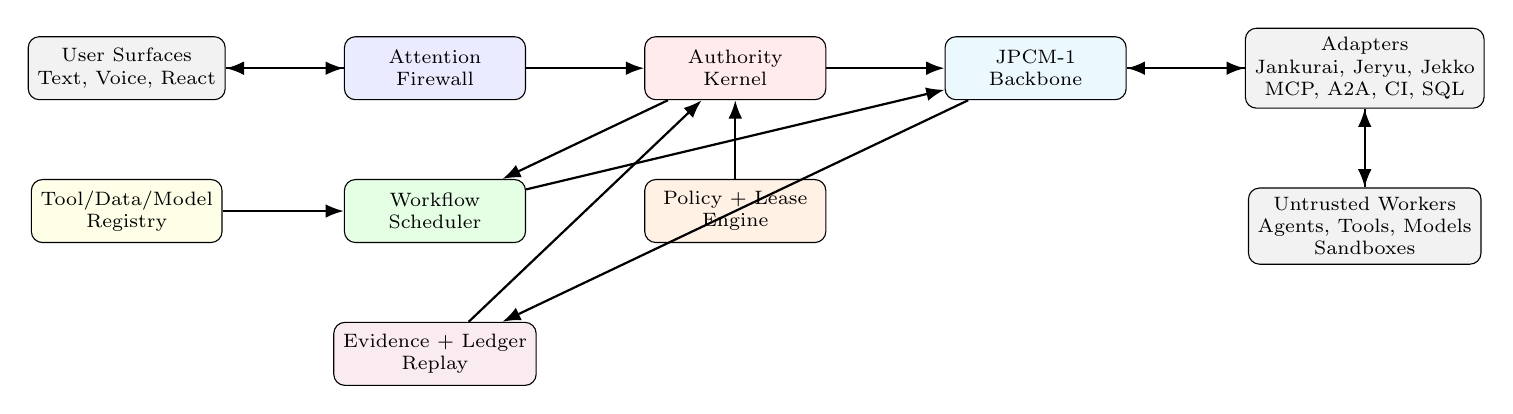
\begin{tikzpicture}[font=\scriptsize, node distance=8mm, box/.style={draw, rounded corners, align=center, minimum height=8mm, minimum width=23mm}, arr/.style={-Latex, thick}]
\node[box, fill=gray!10] (user) {User Surfaces\\Text, Voice, React};
\node[box, right=15mm of user, fill=blue!8] (attention) {Attention\\Firewall};
\node[box, right=15mm of attention, fill=red!8] (authority) {Authority\\Kernel};
\node[box, below=10mm of authority, fill=orange!10] (policy) {Policy + Lease\\Engine};
\node[box, below=10mm of attention, fill=green!10] (workflow) {Workflow\\Scheduler};
\node[box, below=10mm of user, fill=yellow!10] (registry) {Tool/Data/Model\\Registry};
\node[box, below=10mm of workflow, fill=purple!8] (evidence) {Evidence + Ledger\\Replay};
\node[box, right=15mm of authority, fill=cyan!8] (bus) {JPCM-1\\Backbone};
\node[box, right=15mm of bus, fill=gray!10] (adapters) {Adapters\\Jankurai, Jeryu, Jekko\\MCP, A2A, CI, SQL};
\node[box, below=10mm of adapters, fill=gray!10] (workers) {Untrusted Workers\\Agents, Tools, Models\\Sandboxes};
\draw[arr] (user) -- (attention);
\draw[arr] (attention) -- (authority);
\draw[arr] (authority) -- (bus);
\draw[arr] (bus) -- (adapters);
\draw[arr] (adapters) -- (workers);
\draw[arr] (workers) -- (adapters);
\draw[arr] (adapters) -- (bus);
\draw[arr] (bus) -- (evidence);
\draw[arr] (workflow) -- (bus);
\draw[arr] (registry) -- (workflow);
\draw[arr] (policy) -- (authority);
\draw[arr] (authority) -- (workflow);
\draw[arr] (evidence) -- (authority);
\draw[arr] (attention) -- (user);
\end{tikzpicture}
\caption{JMCP reference architecture. The authority kernel is intentionally small. Workers are useful but untrusted. All controlled communication uses JPCM-1.0 envelopes.}
\end{figure*}

JMCP decomposes into seven planes. The Authority Plane owns root decisions, leases, emergency pause, approval gates, signing keys, and policy epochs. The Communication Plane owns JPCM envelopes, subjects, transports, broker bindings, replay, dead-letter queues, and version negotiation. The Workflow Plane owns work orders, task DAGs, scheduling, WIP, budgets, cancellation, and rollback. The Evidence Plane owns receipts, provenance, replay, independent verification, and challenge. The Tool/Data/Model Awareness Plane owns registries, manifests, cost/risk/performance telemetry, and technology radar. The Cognition and Execution Plane contains Jekko/ZYAL, external agents, code tools, CI, browsers, data stores, and generated tools. The User Plane contains text, voice, approvals, digests, drilldown, and the React cockpit.

\section{JPCM-1.0 Protocol}
JPCM-1.0 is a mandatory protocol for all controlled services. It is not tied to a single broker. It has binding profiles for NATS/JetStream, HTTP+JSON, gRPC, WebSocket, stdio adapters, MCP bridges, and A2A bridges. The recommended local-first deployment uses NATS/JetStream because subject-based messaging, request/reply, persistence, replay, key-value storage, and object storage fit JMCP's communication pattern \cite{nats,jetstream}. Large organizations may use Kafka-like logs or replicated ledgers if they preserve JPCM semantics.

\begin{figure}[t]
\centering
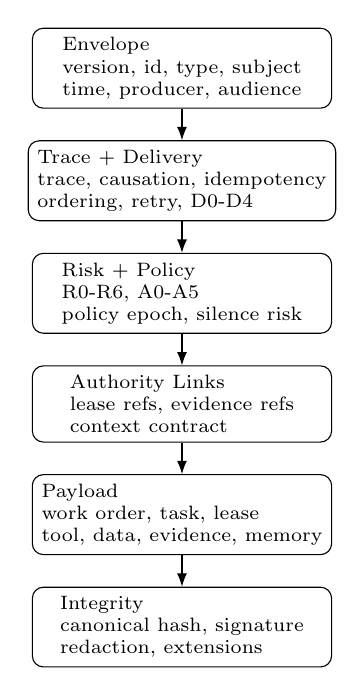
\begin{tikzpicture}[font=\scriptsize, node distance=4mm, box/.style={draw, rounded corners, align=left, minimum width=38mm}]
\node[box] (env) {Envelope\\version, id, type, subject\\time, producer, audience};
\node[box, below=of env] (ctx) {Trace + Delivery\\trace, causation, idempotency\\ordering, retry, D0-D4};
\node[box, below=of ctx] (risk) {Risk + Policy\\R0-R6, A0-A5\\policy epoch, silence risk};
\node[box, below=of risk] (auth) {Authority Links\\lease refs, evidence refs\\context contract};
\node[box, below=of auth] (payload) {Payload\\work order, task, lease\\tool, data, evidence, memory};
\node[box, below=of payload] (sig) {Integrity\\canonical hash, signature\\redaction, extensions};
\draw[-Latex] (env) -- (ctx); \draw[-Latex] (ctx) -- (risk); \draw[-Latex] (risk) -- (auth); \draw[-Latex] (auth) -- (payload); \draw[-Latex] (payload) -- (sig);
\end{tikzpicture}
\caption{Canonical JPCM envelope stack. The protocol binds authority, evidence, risk, delivery, and payload semantics into every message.}
\end{figure}

\subsection{Envelope}
Every envelope contains `jpcm\_version`, `message\_id`, `message\_type`, `subject`, timestamps, producer, optional audience, tenant/workspace/repo identifiers, trace context, delivery semantics, risk context, data classification, policy context, lease references, evidence references, schema reference, payload hash, payload, redaction policy, optional signature, and extensions. Payload hashes are computed over canonical JSON using JCS \cite{jcs}. Signed objects may use JWS, DSSE, Sigstore bundles, or detached signatures \cite{jws,dsse,sigstore}.

\subsection{Delivery Classes}
D0 ephemeral messages may be sampled and dropped. D1 at-most-once messages are advisory. D2 at-least-once messages require idempotency keys. D3 effectively-once messages require dedupe windows and replay-safe handlers. D4 authority-serialized messages require a single authority ordering key and ledger commit before side effect. R6 self-modifying-authority messages must be D4.

\subsection{Message Families}
JPCM-1.0 includes service, intent, voice, attention, work-order, workflow, task, lease, context, tool, data, evidence, policy, fault, incident, memory, self-improvement, research, model, budget, cost, telemetry, and conformance families. This breadth is necessary. A task-management protocol without memory and self-improvement semantics cannot safely support a system that is supposed to always improve. A tool protocol without tool-building proposals cannot manage its own missing capabilities. A voice channel without transcript and confirmation events cannot be a safe authority input.

\subsection{Conformance}
C0 services observe. C1 services report. C2 services act under leases. C3 services produce challengeable evidence. C4 services participate in authority workflows. C5 services propose self-improvement. C5 is not a privilege escalation; it is the most constrained class because it touches the system's future behavior.

\section{Task, Workflow, and Work Orders}
\begin{figure}[t]
\centering
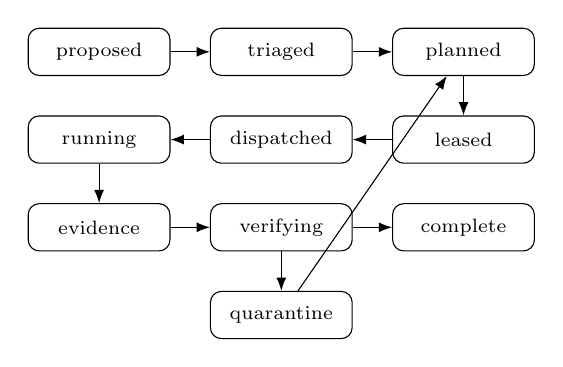
\begin{tikzpicture}[font=\scriptsize, node distance=5mm, state/.style={draw, rounded corners, align=center, minimum width=18mm, minimum height=6mm}, arr/.style={-Latex}]
\node[state] (p) {proposed};
\node[state, right=of p] (t) {triaged};
\node[state, right=of t] (pl) {planned};
\node[state, below=of pl] (l) {leased};
\node[state, left=of l] (d) {dispatched};
\node[state, left=of d] (r) {running};
\node[state, below=of r] (e) {evidence};
\node[state, right=of e] (v) {verifying};
\node[state, right=of v] (c) {complete};
\node[state, below=of v] (q) {quarantine};
\draw[arr] (p)--(t); \draw[arr] (t)--(pl); \draw[arr] (pl)--(l); \draw[arr] (l)--(d); \draw[arr] (d)--(r); \draw[arr] (r)--(e); \draw[arr] (e)--(v); \draw[arr] (v)--(c); \draw[arr] (v)--(q); \draw[arr] (q)--(pl);
\end{tikzpicture}
\caption{Normative task lifecycle. High-risk tasks can move to waiting-for-user, blocked, paused, failed, canceled, rolled-back, or quarantined at any point by policy.}
\end{figure}

A work order is a user or system objective. It contains non-goals, acceptance criteria, budget, attention policy, risk context, and a task DAG. Tasks have kinds, states, owners, dependencies, locks, leases, evidence requirements, rollback references, budgets, and progress. Task kinds include bug fixes, features, refactors, security reviews, incidents, repo creation, research, knowledge compression, memory promotion, tool building, tool audit, self-improvement, telemetry analysis, test generation, dependency updates, performance optimization, cost reduction, policy changes, migrations, releases, rollbacks, documentation, prototypes, sandbox experiments, red-team work, and model evaluations.

The scheduler is portfolio-aware. It deduplicates similar work, imposes WIP limits, honors locks, enforces budgets, routes by cost/risk/latency/reliability, cancels stale tasks, and detects conflicts. It does not maximize activity. It maximizes verified user value per unit risk, cost, and attention.

\section{Capability Leases}
A capability lease is a signed, scoped, revocable authorization for a principal to perform specific actions against specific resources under a specific policy epoch, budget, expiry, and use count. Leases are checked at dispatch and immediately before every side effect. A service that checks leases only once is non-conformant. Lease scopes include repo, path, branch, database, table, cloud account, secret namespace, tool, model, budget, time, network egress, and allowed data class.

Leases solve the confused-deputy problem by making authority explicit. A model can propose an action, but it cannot carry authority merely because it produced text. An adapter can execute a tool, but only if the current lease permits that exact side effect. A self-improvement task can run experiments, but it cannot deploy changes to policy, schema, scheduler, router, sandbox, or authority without quorum and canary.

\section{Evidence and Promotion}
JMCP separates claims from proof. A task's status is a claim. A test log is evidence. A replayable command is stronger evidence. Independent reproduction is stronger still. Evidence bundles bind claims to subject references, artifact hashes, environment descriptions, commands, logs, code hashes, policy epochs, lease identifiers, and producer identities. Evidence quality ranges from E0 claim-only to E5 production-correlated.

Promotion is any durable change to code, configuration, memory, policy, tools, schemas, standards, or production state. No-proof-no-promotion is broader than no-proof-no-merge. A memory can damage future work as much as a bad merge. A tool can become a repeated exploit path. A policy can silently weaken the authority kernel. Therefore evidence gates apply beyond git.

\section{Attention Firewall and Voice}
\begin{figure}[t]
\centering
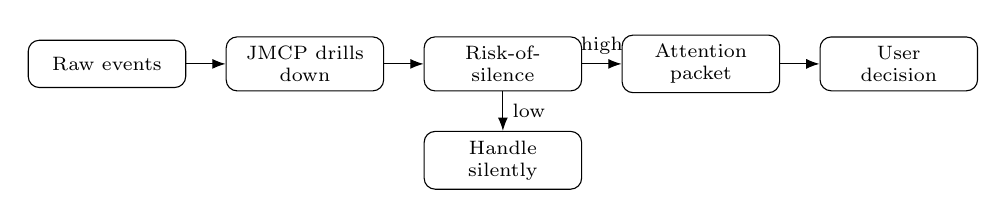
\begin{tikzpicture}[font=\scriptsize, node distance=5mm, box/.style={draw, rounded corners, align=center, minimum width=20mm, minimum height=6mm}]
\node[box] (raw) {Raw events};
\node[box, right=of raw] (diagnose) {JMCP drills\\down};
\node[box, right=of diagnose] (score) {Risk-of-\\silence};
\node[box, below=of score] (silent) {Handle\\silently};
\node[box, right=of score] (packet) {Attention\\packet};
\node[box, right=of packet] (user) {User\\decision};
\draw[-Latex] (raw)--(diagnose); \draw[-Latex] (diagnose)--(score); \draw[-Latex] (score)--node[right]{low}(silent); \draw[-Latex] (score)--node[above]{high}(packet); \draw[-Latex] (packet)--(user);
\end{tikzpicture}
\caption{Attention firewall. The default path is not to ask the user; it is to diagnose, prove, and act within policy unless silence is unsafe.}
\end{figure}

The user's time is a scarce protected resource. JMCP must not solve overload by hiding risk, nor solve risk by interrupting constantly. The attention firewall computes a risk-of-silence score from reversibility, blast radius, uncertainty, user preference, policy, evidence quality, cost, deadline, legal risk, and trust calibration. It escalates only with an attention packet: decision needed, options, recommendation, evidence, cost, rollback, deadline, and drilldown.

Voice input is treated as untrusted until converted into a confirmed intent. Voice can be misheard, spoofed, replayed, captured from background audio, or socially engineered. JPCM represents raw segments, transcript candidates, intent candidates, and confirmation receipts as separate events. R2 and higher voice commands require readback or equivalent confirmation. R4 and higher voice commands require text-visible confirmation or stronger local policy controls. This design preserves the convenience of voice without letting it become a shortcut around authority.

\section{Tool and Data Awareness}
\begin{figure*}[t]
\centering
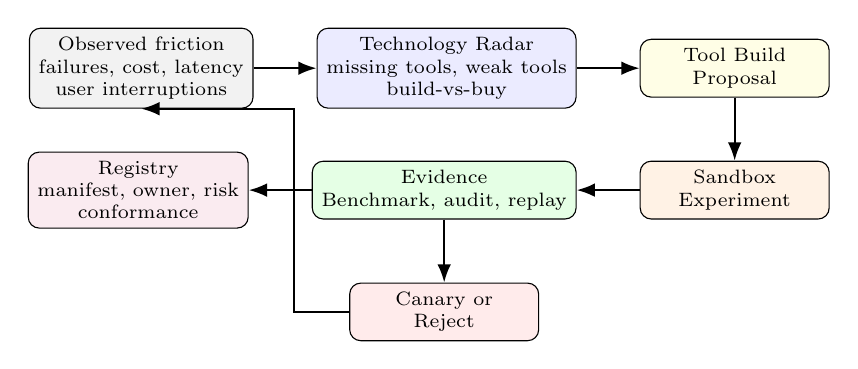
\begin{tikzpicture}[font=\scriptsize, node distance=8mm, box/.style={draw, rounded corners, align=center, minimum width=24mm, minimum height=7mm}, arr/.style={-Latex, thick}]
\node[box, fill=gray!10] (obs) {Observed friction\\failures, cost, latency\\user interruptions};
\node[box, right=of obs, fill=blue!8] (radar) {Technology Radar\\missing tools, weak tools\\build-vs-buy};
\node[box, right=of radar, fill=yellow!10] (proposal) {Tool Build\\Proposal};
\node[box, below=of proposal, fill=orange!10] (sandbox) {Sandbox\\Experiment};
\node[box, left=of sandbox, fill=green!10] (evidence) {Evidence\\Benchmark, audit, replay};
\node[box, left=of evidence, fill=purple!8] (registry) {Registry\\manifest, owner, risk\\conformance};
\node[box, below=of evidence, fill=red!8] (promote) {Canary or\\Reject};
\draw[arr] (obs)--(radar); \draw[arr] (radar)--(proposal); \draw[arr] (proposal)--(sandbox); \draw[arr] (sandbox)--(evidence); \draw[arr] (evidence)--(registry); \draw[arr] (evidence)--(promote); \draw[arr] (promote.west) -- ++(-7mm,0) |- (obs.south);
\end{tikzpicture}
\caption{Tool and data awareness becomes a tool-building loop. JMCP does not only use tools; it decides which tools should exist.}
\end{figure*}

Tool and data awareness is a first-class plane. A manifest records not only what a tool does, but what it touches, what it costs, how fast it is, how often it fails, which leases it requires, which evidence it can produce, who owns it, what SBOM or provenance it has, what sandbox profile it uses, and when it should be deprecated. Data assets have classifications, owners, locations, schemas, freshness, allowed uses, retention classes, lineage, and access policies.

The technology radar is a continuous planning loop. It asks which tools are missing, which tasks repeatedly fail, which user interruptions could be eliminated by better tooling, which repo-local scripts should become global Jankurai standards, which tools have weak evidence, and which model or sandbox upgrades would increase verified yield. Automated tool building is not a side hobby. It is a controlled work class with proposals, manifests, evaluation plans, maintenance owners, sandboxes, evidence, and sunset conditions.

\section{Self-Improvement Governance}
JMCP should always improve, but the phrase ``always improving'' is dangerous unless operationalized. Self-improvement is a hazardous task class. The system may propose changes to prompts, policies, scheduler weights, routing rules, indexes, tools, schemas, UI, observability, sandboxes, and even the authority kernel. The target determines the gate. Measurement-only changes may be automatic. Shadow changes may run without user interruption if they have no side effect. Canary changes require evidence and rollback. Authority-impacting changes require quorum and explicit approval.

A self-improvement proposal includes target, hypothesis, change class, evaluation plan, rollback plan, success metrics, harm metrics, and approval gate. The proposal then runs as a task under JPCM. It cannot rewrite the policy that judges it. It cannot promote itself. It cannot hide harm metrics. It cannot store durable memory without evidence and rollback. If the canary violates harm thresholds, rollback is automatic.

\section{Security Model}
The security model assumes hostile inputs and partial compromise. Prompt injection may be embedded in code, logs, web pages, documentation, tool descriptions, issue comments, test fixtures, and transcripts. Tool poisoning may arrive through MCP or A2A manifests. Memory poisoning may persist a malicious lesson. Evidence spoofing may fake success. CI runners may be compromised. Voice may be spoofed. Adapters may drift or bypass the control plane. The correct posture is not to trust the model less; it is to never make model text the source of authority.

Required controls include minimal trusted computing base, isolated signing keys, revocable leases, D4 authority serialization, sandboxed adapters, manifest signing, SBOM and provenance checks, secret scanning, redaction, evidence challenge, emergency pause, dead-letter queues, immutable ledger, replay, and conformance tests. These controls follow long-standing secure-design principles such as least privilege, fail-safe defaults, complete mediation, economy of mechanism, and separation of privilege \cite{saltzer}.

\section{Communication Backbone and Operations}
The backbone must degrade safely. If the broker is unavailable, low-risk advisory work may pause, but emergency pause, revocation, and critical attention must have redundant paths. If the ledger is unavailable, D4 side effects must stop. If telemetry volume surges, adaptive sampling may reduce D0 events but must not drop leases, policy decisions, evidence bundles, or attention receipts. If clocks drift, expiry validation uses monotonic local checks plus authority-issued timestamps.

Operations must include disaster recovery, replay drills, schema migration rehearsals, key rotation, broker partition tests, corrupted-event tests, stale-lease tests, red-team prompt-injection fixtures, and false-green CI tests. The control plane must be debuggable without assuming the control plane is healthy. This implies offline ledger readers, static schema validators, and manual emergency pause.

\section{React Cockpit}
The React cockpit is not a log viewer. It is an executive process-control surface. The default screen is an Attention Inbox with decisions that truly need the user. Secondary screens show the system map, work graph, evidence drilldown, tool/data radar, voice console, incident room, cost/budget view, and conformance dashboard. The UI should make drilldown fast, but JMCP should perform the first drilldown itself. Human time is spent on judgment, not spelunking.

The frontend should be built with Vite, TypeScript, React, typed clients generated from the JPCM schema, workers for trace indexing, virtualization for large task/evidence lists, and streaming updates over WebSocket or NATS-over-web gateway. It must clearly distinguish claims, evidence, recommendations, uncertainty, and required decisions. It must support text and voice chat without letting chat dominate the architecture.

\section{Evaluation Plan}
A JMCP implementation should be evaluated along five axes. Control correctness measures invalid side effects prevented, stale leases rejected, duplicate commands deduped, and emergency pause latency. Evidence quality measures replay success, independent verification rate, false-green detection, and promotion errors. Attention quality measures interruptions per day, risk-of-silence calibration, missed escalations, user correction rate, and time saved. Tool/data awareness measures registry coverage, tool failure rate, tool-building value, deprecation time, and cost per verified task. Self-improvement safety measures canary rollback correctness, harm detection, and prevention of self-approval.

The most important negative test is not whether the system can do a task. It is whether it refuses to do a task when the lease, evidence, risk, policy, or attention state is wrong. A system that says no correctly is more valuable than a system that acts continuously.

\section{Protocol Schema Summary}
The final deliverable includes `jpcm\_1\_0\_0\_protocol.schema.json`. The schema validates the canonical envelope and all core payload objects. It includes task kinds such as `tool\_build`, `self\_improvement`, `knowledge\_compression`, `memory\_promotion`, `repo\_creation`, `red\_team`, and `model\_eval`. It includes message families for tool building, self-improvement, voice, evidence, data, policy, conformance, and telemetry. It also includes normative rules not fully expressible by JSON Schema, such as lease checks at side-effect time and quorum for authority-impacting self-improvement.

\section{Extreme Future Vector}
JMCP starts as a local-first personal engineering control plane. The extreme future is more ambitious: a sovereign process-intelligence fabric. In that future, JMCP supervises engineering, research, repo creation, incident response, standards evolution, tool marketplaces, data governance, and organizational decision flow. It becomes an engineering digital twin that understands bottlenecks, yield, risk, dependencies, costs, missing tools, weak standards, and user attention. It can create new repos, create new tools, compress knowledge, run experiments, build benchmarks, and federate evidence with other organizations without exposing sensitive internals.

The ambition is intentionally large, but the guardrail is strict: autonomy may expand only when evidence, containment, observability, and attention quality expand faster. This is the difference between a useful autonomous engineering fab and an uncontrolled agent swarm.


\section{Final Rubric as Engineering Requirements}
The scoring rubric used in the review is intentionally more severe than a normal architecture review. A normal review asks whether the system is understandable. This review asks whether independent implementers could build interoperable services that remain safe when agents, tools, evidence, memory, and users are all imperfect. The rubric therefore becomes a requirements document.

\subsection{Definition and Negative Definition}
The system must be defined by ownership. JMCP owns authority, leases, work orders, task state, policy decisions, evidence acceptance, memory promotion, tool adoption, self-improvement gates, and user attention. It does not own every implementation detail of every agent or tool. The negative definition is equally important because most failures start as category confusion: a team treats a coding agent as the authority, a dashboard as observability, CI as proof, chat as the product, or MCP as a safety model. JMCP must reject these shortcuts.

\subsection{Authority and Containment}
Authority is a runtime property, not a documentation property. A service is not trusted because it is in the repository, signed once, or has a friendly manifest. It is trusted only to the degree allowed by its current lease, policy epoch, sandbox, data scope, budget, and evidence obligations. This means every adapter must mediate side effects. A shell command, git push, database write, cloud API call, production deployment, memory write, policy change, schema update, or generated tool install is a side effect. The adapter is non-conformant if it lets the worker act directly.

\subsection{Protocol Normativity}
A protocol is not normative until two independent teams can implement it, exchange messages, reject invalid messages for the same reasons, replay the same events, and pass the same conformance fixtures. JPCM-1.0 therefore specifies envelope fields, payload objects, message families, delivery classes, risk tiers, autonomy tiers, data classes, signatures, redaction, idempotency, ordering, error codes, task states, and conformance levels. The JSON schema is necessary but not sufficient. Normative rules outside JSON Schema are also part of the standard.

\subsection{Task and Workflow Completeness}
A control plane without a rich task model becomes a queue. JMCP needs a portfolio scheduler, not a TODO list. It must manage dependencies, locks, WIP limits, budgets, retries, cancellation, rollback, uncertainty, evidence requirements, dedupe, conflict detection, and escalation. It must support ordinary engineering work and meta-work: memory promotion, knowledge compression, tool audit, tool build, self-improvement, model evaluation, red-team work, technology radar, and policy change.

\subsection{Security}
The security rubric assumes the control plane is a high-value target. The correct question is not whether the model is aligned. The correct question is what damage occurs when the model is wrong, the tool is poisoned, the transcript is spoofed, the CI runner is compromised, the memory is corrupted, or the adapter is stale. A strong design contains each failure and preserves enough evidence to recover.

\subsection{Evidence and Certification}
Evidence must be typed, replayable, and challengeable. A log line is not the same as a reproducible test. A model summary is not the same as a proof. A screenshot is not the same as a signed attestation. Evidence is accepted at levels E0 through E5. Promotion policies specify minimum levels for each action class. JMCP must be able to say: this claim is plausible but not promotable.

\subsection{Tool and Data Awareness}
Tool awareness is not an inventory spreadsheet. It is an operating model for improving the system. JMCP must know which tools exist, which tasks use them, how often they fail, what they cost, what data they touch, what leases they require, what evidence they produce, what alternatives exist, and whether they should be replaced or built. Data awareness similarly tracks classification, owner, freshness, retention, allowed uses, lineage, and access history.

\subsection{User Attention}
The user is not a human interrupt handler. JMCP must prove that interruption is necessary. Every escalation includes the reason, options, recommendation, evidence, cost, risk, rollback, deadline, and drilldown. If the system cannot produce that packet, it probably has not investigated deeply enough. The bare-minimum interface is not minimal because it hides information; it is minimal because the system does the investigative work first.

\section{JPCM-1.0 Normative Rules}
This section states the protocol rules in implementation language. The schema file is the machine-readable companion; these rules are the semantic standard.

\begin{longtable}{p{0.08\textwidth}p{0.84\textwidth}}
\caption{Core JPCM-1.0 normative rules.}\\
\toprule
ID & Rule\\
\midrule
N1 & Every controlled participant MUST publish a ServiceManifest before performing controlled work.\\
N2 & Every controlled message MUST validate against the JPCM-1.0 envelope schema or be quarantined as external input.\\
N3 & Required envelope fields MUST NOT be reinterpreted by extensions.\\
N4 & Payload hashes MUST be computed from canonical JSON using JCS unless the binding profile defines a stronger canonicalization.\\
N5 & Authority, lease, evidence, memory, policy, self-improvement, and tool-build messages MUST be signed.\\
N6 & Side-effecting messages MUST include a valid CapabilityLease reference.\\
N7 & Adapters MUST revalidate leases immediately before execution, not merely when work is dispatched.\\
N8 & A lease MUST be bound to principal, capability, scope, policy epoch, expiry, and budget.\\
N9 & Revocation MUST propagate through a D4 authority-serialized event.\\
N10 & R4, R5, and R6 risk messages SHOULD use D4 delivery; R6 messages MUST use D4 delivery.\\
N11 & Duplicate D2/D3/D4 messages MUST be deduplicated by idempotency key.\\
N12 & A handler MUST be safe under replay for its declared delivery class.\\
N13 & State changes MUST be monotonic except for explicit rollback, quarantine, or policy-authorized replan transitions.\\
N14 & Work orders MUST contain objective, non-goals, risk, tasks, acceptance criteria, budget, and attention policy.\\
N15 & Tasks MUST declare kind, state, owner, dependencies, required leases, evidence requirements, and rollback plan where applicable.\\
N16 & A task MUST NOT enter ready-to-promote unless required evidence exists and verifies under the current policy epoch.\\
N17 & Evidence bundles MUST bind claims to subject references, artifact hashes, producer, environment, policy epoch, and lease references when applicable.\\
N18 & Evidence MAY be challenged; challenge outcomes MUST be recorded.\\
N19 & E0 evidence MUST NOT promote durable code, memory, policy, tools, or production state.\\
N20 & Memory promotion MUST include scope, claim, evidence, confidence, TTL, counterexamples, and rollback.\\
N21 & Global memory promotion SHOULD require stronger evidence than repo-local memory promotion.\\
N22 & Tool use MUST be preceded by a ToolManifest, audit result, sandbox profile, and conformance claim.\\
N23 & Tool manifests MUST declare side-effect class, data touched, required leases, cost model, and evidence outputs.\\
N24 & Data assets MUST declare classification, owner, location, freshness, allowed uses, retention, and lineage.\\
N25 & Data classification MUST flow through derived artifacts unless downgraded by an explicit redaction policy.\\
N26 & Voice segments MUST become transcript candidates before intent candidates.\\
N27 & R2+ voice-originated intents MUST require readback or equivalent explicit confirmation.\\
N28 & R4+ voice-originated intents MUST require text-visible confirmation or stronger local policy.\\
N29 & User escalations MUST be represented as AttentionPackets.\\
N30 & AttentionPackets MUST include decision, options, recommendation, evidence summary, cost/risk consequence, deadline, and drilldown refs.\\
N31 & Self-improvement proposals MUST include target, hypothesis, change class, evaluation plan, rollback plan, success metrics, harm metrics, and approval gate.\\
N32 & Self-improvement that touches policy, schema, scheduler, router, sandbox, or authority MUST require quorum.\\
N33 & A self-improvement task MUST NOT approve or promote itself.\\
N34 & Generated tools MUST start in quarantine or sandbox-only mode.\\
N35 & Tool-building proposals MUST include expected value, risk, evaluation plan, maintenance owner, and sunset condition.\\
N36 & Emergency pause MUST stop new D4 side effects and revoke active high-risk leases.\\
N37 & Dead-lettered authority messages MUST create an incident.\\
N38 & Services MUST emit heartbeat and conformance status.\\
N39 & A bridge from MCP, A2A, OpenClaw, or any external protocol MUST translate into JPCM and MUST NOT bypass policy.\\
N40 & External tool descriptions MUST be treated as untrusted data even when signed.\\
N41 & Payloads containing credentials MUST be rejected or redacted according to policy.\\
N42 & Every schema migration MUST include compatibility tests and rollback.\\
N43 & A service that cannot support the required conformance level MUST be downgraded or quarantined.\\
N44 & The ledger MUST preserve enough information to replay decisions, not merely reconstruct display logs.\\
N45 & The cockpit MUST distinguish claims from evidence.\\
N46 & Cost and budget events MUST be attributable to work order, task, model, tool, and lease when possible.\\
N47 & Policy decisions MUST record policy epoch, ruleset refs, decision, reason, and obligations.\\
N48 & Incident records MUST include timeline, blast radius, containment, evidence, rollback, and lessons proposed.\\
N49 & Technology-radar recommendations MUST be evidence-backed before becoming tool-build tasks.\\
N50 & Federation MUST NOT export raw sensitive evidence unless an explicit sharing policy permits it.\\
\bottomrule
\end{longtable}

\section{Message Family Semantics}
The JPCM message families are designed to prevent the most common ambiguity in multi-agent systems: conflating a request, a claim, an authorization, an observation, and a proof. A request asks for something. A command authorizes a specific action under a lease. An event states that something happened. Evidence supports or contradicts a claim. A policy decision allows, denies, quarantines, or requires more evidence. An attention packet asks the user to decide. Each family exists to preserve these distinctions.

\begin{longtable}{p{0.16\textwidth}p{0.30\textwidth}p{0.44\textwidth}}
\caption{JPCM message families and their reason for existence.}\\
\toprule
Family & Example message types & Purpose\\
\midrule
Service & service.manifest.published, service.heartbeat, service.degraded & Declare identity, health, interfaces, conformance, and trust tier.\\
Intent & intent.submitted, user.message, research.query.created & Capture human, system, scheduled, or research objectives before work-order creation.\\
Voice & voice.segment.created, voice.transcript.candidate, voice.intent.candidate & Preserve modality-native evidence and prevent voice from bypassing confirmation.\\
Attention & attention.packet.created, approval.requested, approval.decision.recorded & Manage minimum-safe user interruption and auditable approvals.\\
Work & work\_order.created, workflow.graph.created, task.created & Represent objectives, task graphs, dependencies, and scheduler state.\\
Task events & task.state.changed, task.progress.reported, task.completed, task.failed & Track runtime state without confusing status claims with proof.\\
Lease & lease.requested, lease.issued, lease.revoked, context.contract.granted & Convert authority into scoped, revocable runtime permission.\\
Tool & tool.manifest.published, tool.call.requested, tool.call.result, tool.build.proposed & Govern existing tools and the creation of new tools.\\
Data & data.asset.registered, data.access.requested, data.observation.recorded & Track data assets, classification, freshness, allowed use, and access decisions.\\
Evidence & evidence.bundle.created, evidence.verification.result, evidence.challenge.created & Bind claims to artifacts, provenance, replay, and challenge.\\
Policy & policy.decision.recorded, policy.violation.detected & Make decisions and violations explicit and replayable.\\
Memory & memory.candidate.created, memory.accepted, memory.revoked & Treat durable learning as governed change, not hidden summarization.\\
Self & self\_improvement.proposed, self\_improvement.canary.started, self\_improvement.rolled\_back & Allow improvement while preventing the judged component from rewriting the judge.\\
Telemetry & telemetry.emitted, budget.event.recorded, cost.event.recorded & Attribute cost, latency, traces, and health to work and decisions.\\
Conformance & conformance.result.recorded & Certify that implementations respect schema, semantics, and failure behavior.\\
\bottomrule
\end{longtable}

\section{Risk, Autonomy, and Delivery Classes}
Risk tiers classify blast radius. Autonomy tiers classify how far an agent may proceed. Delivery classes classify message reliability and ordering. These are independent fields because a low-risk task can still require reliable delivery, and a high-risk task can be allowed only in draft mode.

\begin{longtable}{p{0.12\textwidth}p{0.30\textwidth}p{0.48\textwidth}}
\caption{Risk tiers.}\\
\toprule
Tier & Name & Meaning\\
\midrule
R0 & Read-only & Inspection, search, summarization, local analysis without side effects.\\
R1 & Local draft & Local file drafts, throwaway experiments, no repo or secret impact.\\
R2 & Repo draft & Branches, PR drafts, tests, docs, repo-local scripts.\\
R3 & Cross-repo & Shared standards, generated global tools, multi-repo refactors, shared memory.\\
R4 & Production or secret & Production calls, credentials, regulated data, customer data, deployment, billing.\\
R5 & Policy or memory & Durable memory, global lessons, tool adoption, policy, evidence rules.\\
R6 & Self-modifying authority & Authority kernel, schema, scheduler, router, sandbox, signing, emergency pause.\\
\bottomrule
\end{longtable}

\begin{longtable}{p{0.12\textwidth}p{0.30\textwidth}p{0.48\textwidth}}
\caption{Autonomy tiers.}\\
\toprule
Tier & Name & Meaning\\
\midrule
A0 & Human-only & JMCP may analyze but not act.\\
A1 & Suggest & JMCP may propose plans and ask.\\
A2 & Draft & JMCP may create drafts, branches, evidence, or simulations.\\
A3 & Act with lease & JMCP may execute bounded side effects under lease.\\
A4 & Act with proof & JMCP may promote low/mid-risk changes if evidence gates pass.\\
A5 & Shadow or canary only & Used for self-improvement and new tools before broad promotion.\\
\bottomrule
\end{longtable}

\section{Lease Lifecycle}
A lease starts as a request. The policy engine evaluates principal, task, requested capability, scope, data class, risk, autonomy tier, budget, expiry, policy epoch, recent incidents, and tool conformance. It returns allow, deny, require-human, require-more-evidence, quarantine, or require-quorum. If allowed, the authority kernel issues a signed lease. The lease may be used only by the bound principal, for the bound task, within the bound scope, before expiry, under budget, and under the issuing policy epoch. The adapter checks the lease immediately before each side effect. A revocation event invalidates the lease even if the worker has not observed it; adapters must consult the authority or local revocation cache before executing high-risk side effects.

Lease design prevents ambient authority. It also gives the user and system a way to stop work without killing every process. Emergency pause is implemented as broad revocation plus refusal to issue new high-risk leases. Low-risk read-only diagnosis may continue so the system can explain what is happening.

\section{Data Governance and Redaction}
JPCM messages carry data classification because data boundaries are harder than repo boundaries. A task may begin as public documentation but touch confidential architecture, credentials, customer traces, or regulated data. Classification must propagate into derived evidence, summaries, memory candidates, and tool-build artifacts. Redaction is not cosmetic. It determines which principals can view a payload, how long it is retained, whether it can be exported, whether it can be used for model context, and whether it can enter global memory.

A data asset record includes owner, location, schema, freshness, allowed uses, retention class, and lineage. Access is granted through context contracts and leases. A context contract is a scoped grant to use data for a purpose. It is not a raw database credential. It can require aggregation, redaction, differential access, or local-only processing. Evidence bundles must be scanned for secrets before storage, and redacted artifacts must keep links to sealed originals when allowed by policy.

\section{Examples of Controlled Workflows}
\subsection{Routine Bug Fix}
A user says: ``fix the flaky login test.'' JMCP creates an intent, queries Jeryu for code graph context, checks Jankurai standards, asks Jekko or another coding agent for a plan, issues a repo-draft lease, creates a branch, runs tests, collects evidence, and opens a PR draft. If evidence meets policy and the change is low risk, JMCP may summarize completion without interrupting. If the flaky test hides a security regression, the risk tier rises and the user gets an attention packet.

\subsection{Security-Sensitive Change}
A dependency update touches authentication. JMCP creates tasks for dependency analysis, changelog review, vulnerability review, test generation, sandbox execution, and evidence verification. It issues narrow leases. It requires stronger evidence: static analysis, tests, lockfile diff, SBOM update, and independent replay. It escalates before merge because blast radius includes secrets and production identity.

\subsection{Automated Tool Building}
JMCP observes that five repos repeatedly need the same migration checker. The technology radar proposes a global tool. A `tool.build.proposed` message includes expected value, risks, evaluation plan, maintenance owner, and sunset condition. The tool is generated in sandbox, audited by Jankurai, tested against historical migrations from Jeryu, and canaried on one repo. Only after evidence passes does the tool become a certified global Jankurai tool.

\subsection{Memory Promotion}
A task discovers that a library version causes false-positive security reports. The agent proposes a memory. JMCP records the claim, evidence, counterexamples, confidence, TTL, and scope. If the problem is repo-local, the memory may be accepted for that repo. If it is global, JMCP requires stronger evidence across repositories and a rollback path. The memory is never silently promoted from a chat summary.

\subsection{Self-Improvement}
JMCP notices that the scheduler creates too many parallel low-value tasks. It proposes a scheduler-weight change. The change runs in shadow mode against replayed historical workloads. Harm metrics include missed high-risk escalations, longer time to critical fix, increased cost, and lower evidence quality. If shadow results improve, a canary may run on low-risk tasks. The scheduler cannot approve its own deployment.

\section{Conformance and Test Strategy}
The conformance suite is as important as the schema. It contains valid fixtures for every message type, invalid fixtures for missing fields and forbidden combinations, replay tests, duplicate tests, stale-lease tests, signature tests, redaction tests, schema migration tests, voice ambiguity tests, tool poisoning tests, memory poisoning tests, evidence spoofing tests, and self-improvement rollback tests. A service claims C0 through C5 only by passing the corresponding suite.

\begin{longtable}{p{0.20\textwidth}p{0.32\textwidth}p{0.38\textwidth}}
\caption{Conformance test categories.}\\
\toprule
Category & Positive test & Negative test\\
\midrule
Envelope & Valid signed payload accepted & Missing schema ref rejected\\
Canonical hash & JCS hash matches payload & Whitespace-equivalent malicious payload rejected if hash differs\\
Lease & Scoped lease permits exact side effect & Stale, over-scope, expired, revoked lease rejected\\
Delivery & Duplicate D3 event deduped & Duplicate PR/migration prevented\\
Ordering & D4 serialized events replay deterministically & Out-of-order authority event quarantined\\
Task state & Legal transition accepted & Promotion without evidence rejected\\
Evidence & Replayable evidence accepted & Screenshot-only promotion rejected\\
Voice & Readback creates approval receipt & R4 voice command without confirmation rejected\\
Tool & Certified tool call executed & Unsigned tool manifest quarantined\\
Memory & Scoped memory with TTL accepted & Global memory without counterexamples rejected\\
Self-improvement & Shadow/canary/rollback works & Policy self-modification without quorum rejected\\
Backpressure & D0 telemetry sampled safely & D4 lease revocation never dropped\\
\bottomrule
\end{longtable}

\section{Deployment Topology}
A minimal local deployment has one authority daemon, one NATS/JetStream server, one SQL database, one object store, one policy engine, one scheduler, one evidence service, one registry, one attention service, and one React cockpit. Adapters run as separate processes with constrained credentials. Workers run in sandboxed processes, containers, VMs, or WebAssembly runtimes depending on risk. Voice and channel surfaces are external input adapters, not authority.

A resilient deployment separates the authority kernel from the broker and ledger, uses replicated storage, rotates keys, enforces network policies, maintains offline schema validators, and provides a manual emergency pause path. A multi-tenant deployment isolates tenants at policy, ledger, object store, secret, and broker-subject levels. A federated deployment exchanges signed evidence summaries rather than raw sensitive artifacts.

\section{Performance and Memory Use}
The implementation should be engineered as a control system, not a bulk logging pipeline. D0 telemetry is sampled and aggregated. D1/D2 events are retained according to operational value. D3/D4 events, evidence bundles, policy decisions, leases, approvals, and memory changes are retained with stronger guarantees. The cockpit should use virtualization, incremental indexes, and worker threads for trace graph operations. The authority kernel should keep a small hot state: active leases, revocation cache, policy epoch, emergency pause state, and open D4 ordering keys.

Backpressure is explicit. When queues grow, JMCP reduces low-risk exploration, cancels duplicate research, pauses non-urgent tool-building tasks, increases summarization, and preserves authority traffic. The correct failure mode is reduced autonomy, not lost control.

\section{Research and Validation Agenda}
The research agenda has practical and scientific components. Practically, JMCP needs benchmarks for verified work per user interruption, evidence quality per dollar, false promotion rate, missed escalation rate, task dedupe efficiency, tool-building return on investment, and self-improvement harm detection. Scientifically, JMCP creates a setting for studying protocol-governed autonomy: how to combine model reasoning, formal policy, evidence, human attention, and distributed systems into reliable agentic workflows.

Key open questions include: how to measure risk-of-silence, how to detect evidence theater, how to prevent memory poisoning at scale, how to compare generated tools to human-built tools, how to route multimodal context without leaking sensitive data, how to federate evidence without revealing proprietary details, and how to prove that self-improvement is making the control plane safer rather than merely more active.

\section{Product Requirements for the Extreme Future}
The extreme vector is not vague futurism if converted into requirements. The personal engineering control room requires text, voice, attention packets, repo visibility, and safe autonomous work. The software fab requires standards, proof lanes, scheduling, and continuous maintenance. Cross-repo process intelligence requires scoped memory, knowledge compression, and data governance. The R\&D foundry requires research, prototype generation, benchmarks, and repo creation. The proof-carrying tool marketplace requires signed manifests, SBOMs, evaluation, canary, and deprecation. The engineering digital twin requires graph models of code, work, evidence, incidents, cost, and bottlenecks. The self-hardening organization OS requires careful expansion beyond engineering while preserving the same lease/evidence/attention laws.


\section{Conclusion}
JMCP and JPCM-1.0 define a protocol-first answer to agentic engineering control. The core insight is that the primary interface should not expose all activity; it should absorb activity, diagnose it, prove it, and reveal only what the user must decide. The protocol is the mechanism that keeps this honest. Every service speaks the same envelope, every side effect requires a lease, every claim requires evidence, every durable lesson requires provenance, every risky user interruption requires an attention packet, and every self-improvement runs through canary and rollback. This is not a chatbot with tools. It is a control plane for making agentic work safe, observable, ambitious, and worth the user's time.

\appendices
\section{Normative JPCM Object Families}
This appendix summarizes the object families implemented in the JSON schema. Service manifests define service identity, interfaces, capabilities, touched data, side effects, trust requirements, sandbox profile, SBOM reference, SLSA level, and conformance claim. Work orders define objectives, non-goals, risk, tasks, acceptance criteria, budgets, and attention policy. Tasks define kind, state, owner, dependencies, locks, leases, evidence requirements, rollback, budget, and progress. Workflow graphs define nodes, edges, WIP limits, and scheduler. Capability leases define principal, capabilities, scope, constraints, expiry, use count, policy epoch, and revocation subject. Tool manifests define inputs, outputs, side-effect class, risk, cost, latency, required leases, and deprecation. Evidence bundles define claims, subject references, items, evidence quality, verdict, and replay commands. Attention packets define the user decision, options, recommendation, evidence context, deadline, and drilldown. Voice segments define source, transcript, confidence, speaker verification, ambient risk, and confirmation requirements. Memory proposals define scope, claim, evidence, confidence, TTL, counterexamples, rollback, and promotion gate. Tool-build and self-improvement proposals define hypotheses, risk, evaluation, owners, harm metrics, success metrics, and rollback.

\section{Failure Catalogue}
The final design is driven by expected failures. Authority can collapse through bypass, ambient credentials, or self-modifying policy. Protocols can drift through unversioned payloads and missing semantics. Agents can fail through prompt injection, hidden tool instructions, or long-horizon drift. Evidence can become theater through spoofed CI, fake logs, screenshots, or non-replayable tests. Memory can poison future tasks. Tool registries can lie about side effects. Voice can be spoofed or misheard. Telemetry can overwhelm storage. The cockpit can become noise. The future vector can become vague futurism. Each failure maps to a protocol field, policy rule, conformance test, or attention gate.

\section{Implementation File Tree}
The implementation should use Rust crates for authority, JPCM types, bus bindings, ledger, policy, scheduler, attention, registry, evidence, memory, self-improvement, sandbox, and adapters. The React UI should be generated from typed schema clients and organized around attention, system map, task graph, evidence, tool radar, and voice. Conformance fixtures should include valid and invalid envelopes, prompt-injection samples, tool-poisoning manifests, stale leases, bad signatures, hash mismatches, false-green CI, voice ambiguity, memory contradictions, and self-improvement rollback cases.


\section{Expanded Failure-to-Control Matrix}
The following matrix is intentionally long. A control plane for autonomous engineering should be designed against boring, repeated failures as much as exotic attacks. Each row is a failure that must become a fixture, alert, policy rule, or conformance condition.

\begin{longtable}{p{0.22\textwidth}p{0.34\textwidth}p{0.34\textwidth}}
\caption{Failure-to-control matrix.}\\
\toprule
Failure & How it appears & Required controls\\
\midrule
Direct write bypass & Adapter or tool writes to git, SQL, cloud, or production without JPCM & Gateway credentials only, network egress deny, lease audit, canary bypass tests\\
Ambient credential creep & Long-lived tokens remain inside workers & Lease-scoped token minting, vault broker, token TTL, secret scanner\\
Stale lease replay & Old lease used after policy or scope changes & Policy epoch binding, revocation cache, D4 ordering, replay tests\\
Self-approval & Self-improvement modifies its own judge & Quorum gate, separate evaluator, immutable evaluation plan\\
Emergency pause miss & Running workers continue after pause & Revocation broadcast, adapter preflight, kill switch, pause drill\\
Schema drift & Services emit similar but incompatible payloads & Schema registry, conformance suite, compatibility gates\\
Duplicate side effect & Retry creates duplicate PR, migration, email, or deployment & Idempotency keys, dedupe windows, effect receipts\\
Out-of-order authority & Revocation arrives after execution & D4 ordering keys, adapter authority checks, local revocation cache\\
Lost evidence & Backpressure drops proof artifacts & Priority streams, object-store write-through, no-drop evidence class\\
Poisoned tool description & Tool manifest hides prompt injection & Manifest quarantine, human-visible diff, tool-description sanitizer\\
Lookalike tool & Malicious tool mimics trusted tool name & Signed service ids, trust store, registry pinning\\
Compromised CI runner & Runner fabricates green tests & Independent replay, runner attestation, random verifier\\
Evidence theater & Screenshots/logs replace proof & Evidence quality policy, challenge, promotion minimums\\
False green tests & Tests pass while bug persists & Mutation tests, historical regression replay, coverage gates\\
Non-replayable proof & Dependency or environment disappears & Pinned artifacts, SBOM, container digest, object-store copies\\
Memory poisoning & Bad lesson becomes durable global memory & Memory evidence, TTL, counterexamples, scope, rollback\\
Memory overgeneralization & Local workaround becomes global rule & Scope gate, cross-repo evidence, confidence decay\\
Contradictory memory & Compression hides conflict & Contradiction index, memory challenge, provenance retention\\
Voice spoofing & Attacker replays or imitates user & Readback, liveness, text confirmation for R4+, physical-presence policy\\
Voice misrecognition & Transcript changes intent & Confidence threshold, transcript display, ambiguity packet\\
Attention overload & User stops reading alerts & Risk-of-silence score, interruption budget, digest mode\\
Attention underload & System hides important decision & Missed-escalation tests, incident review, calibration metrics\\
Cost runaway & Parallel agents spend without value & Budgets, WIP limits, cost events, cancellation policy\\
Telemetry explosion & Observability costs dominate & Adaptive sampling, causal compression, retention tiers\\
Control-plane dependency loop & JMCP needs itself to debug itself & Offline validators, ledger reader, manual pause\\
Model overtrust & Model summary accepted as truth & Claims/evidence separation, independent verification\\
Router misclassification & Cheap model gets high-risk task & Risk-aware routing, policy gate, model eval telemetry\\
Sandbox escape & Worker escapes container or VM & Defense-in-depth, egress controls, ephemeral runners, host hardening\\
Data leak through evidence & Proof bundle stores secrets & Secret scan, redaction, sealed evidence, classification flow\\
License leak & Cross-repo memory copies incompatible code & License classifier, provenance refs, allowed-use policy\\
Federation leak & External org receives sensitive evidence & Evidence summaries, policy sharing, encrypted selective disclosure\\
Generated tool rot & Built tool remains unowned & Maintenance owner, sunset condition, deprecation event\\
Tool sprawl & System builds tools faster than audits & Tool-building budget, registry review, value threshold\\
Unbounded research & Research tasks never terminate & Hypothesis, budget, stopping rule, summary artifact\\
Task conflict & Two agents modify same file or dependency & Locks, DAG conflict detection, branch isolation\\
Priority inversion & Low-risk tasks block incident work & Risk-first preemption, WIP partitioning\\
Silent policy weakening & Policy update lowers safeguards & Policy diff, quorum, evidence, canary\\
Schema weakening & New schema makes malicious field legal & Schema review, negative fixtures, extension constraints\\
UI deception & Cockpit shows status without evidence & Claim/evidence visual separation, evidence drilldown\\
Stale registry & Registry says tool is healthy when it is not & Heartbeat, conformance expiry, runtime telemetry\\
Data freshness illusion & Recent modified time mistaken for truth & Content provenance, freshness field, source quality\\
Incident without learning & Same failure repeats & Post-incident memory proposal, tool radar, counterexample tracking\\
Learning without incident & Spurious lesson from one event & Evidence threshold, scope, TTL\\
Overfitting self-improvement & Optimizer improves benchmark only & Holdout workloads, harm metrics, user-value metrics\\
Canary blindness & Canary lacks real risk conditions & Representative canary, shadow replay, production-correlated metrics\\
Clock skew & Expiry and ordering fail & Authority timestamps, monotonic timers, skew detection\\
Dead-letter invisibility & Failed messages are ignored & Dead-letter incident creation, retry policy\\
Approval ambiguity & User approves without understanding & Attention packet options, consequences, rollback\\
Human rubber stamp & Too many approvals train bad behavior & Ask less, prove more, confidence calibration\\
Bridge trust inflation & MCP/A2A tools treated as native & Bridge quarantine, manifest translation, conformance class\\
External API drift & Tool behavior changes silently & Contract tests, version pinning, observation alerts\\
Partial outage unsafe & System continues high-risk work without ledger & D4 stop-on-ledger-fail, degraded mode\\
Ledger corruption & History cannot be trusted & Append-only signatures, snapshots, backups, audit verification\\
Policy/ledger mismatch & Decision refers to unavailable policy epoch & Policy bundle hash retention, replay bundle\\
Secret in prompt & Agent context includes credentials & Prompt redaction, secret broker, no-secret contexts\\
Prompt injection detector bypass & LLM defense is treated as sufficient & Least privilege, tool separation, evidence gate\\
Unbounded context sharing & Agents see unrelated sensitive data & Context contracts, data minimization, retrieval policy\\
Wrong negative definition & Team ships assistant instead of control plane & Architecture review, acceptance criteria, authority tests\\
Overcentralization & Control plane becomes single catastrophic target & Small TCB, separation, key isolation, recovery drills\\
Undercentralization & Authority splits between tools and agents & No-bypass law, gateway credentials, audit\\
\bottomrule
\end{longtable}

\section{Complete Message Type Universe}
The schema includes the following message types. Future versions may add types, but conforming 1.0.0 services must not invent semantics for missing core families. Unknown extension types must be quarantined unless explicitly enabled by policy.

\begin{longtable}{p{0.08\textwidth}p{0.54\textwidth}p{0.28\textwidth}}
\caption{JPCM-1.0.0 message type universe.}\\
\toprule
No. & Message type & Family\\
\midrule
1 & service.manifest.published & service\\
2 & service.heartbeat & service\\
3 & service.degraded & service\\
4 & service.retired & service\\
5 & service.capability.changed & service\\
6 & intent.submitted & intent\\
7 & user.message & user\\
8 & voice.segment.created & voice\\
9 & voice.transcript.candidate & voice\\
10 & voice.intent.candidate & voice\\
11 & attention.candidate & attention\\
12 & attention.packet.created & attention\\
13 & attention.escalation.created & attention\\
14 & attention.receipt.recorded & attention\\
15 & approval.requested & approval\\
16 & approval.decision.recorded & approval\\
17 & work\_order.created & work\_order\\
18 & work\_order.updated & work\_order\\
19 & workflow.graph.created & workflow\\
20 & workflow.graph.updated & workflow\\
21 & workflow.graph.closed & workflow\\
22 & task.created & task\\
23 & task.commanded & task\\
24 & task.state.changed & task\\
25 & task.progress.reported & task\\
26 & task.blocked & task\\
27 & task.unblocked & task\\
28 & task.cancel.requested & task\\
29 & task.rollback.requested & task\\
30 & task.completed & task\\
31 & task.failed & task\\
32 & task.quarantined & task\\
33 & lease.requested & lease\\
34 & lease.issued & lease\\
35 & lease.denied & lease\\
36 & lease.renewed & lease\\
37 & lease.revoked & lease\\
38 & lease.expired & lease\\
39 & context.contract.granted & context\\
40 & context.contract.revoked & context\\
41 & tool.manifest.published & tool\\
42 & tool.audit.requested & tool\\
43 & tool.audit.result & tool\\
44 & tool.call.requested & tool\\
45 & tool.call.authorized & tool\\
46 & tool.call.denied & tool\\
47 & tool.call.result & tool\\
48 & tool.build.proposed & tool\\
49 & tool.build.plan.created & tool\\
50 & tool.build.result & tool\\
51 & tool.deprecated & tool\\
52 & tool.decommissioned & tool\\
53 & data.asset.registered & data\\
54 & data.asset.updated & data\\
55 & data.access.requested & data\\
56 & data.access.granted & data\\
57 & data.access.denied & data\\
58 & data.observation.recorded & data\\
59 & evidence.bundle.created & evidence\\
60 & evidence.item.appended & evidence\\
61 & evidence.verification.requested & evidence\\
62 & evidence.verification.result & evidence\\
63 & evidence.challenge.created & evidence\\
64 & policy.decision.recorded & policy\\
65 & policy.violation.detected & policy\\
66 & fault.detected & fault\\
67 & incident.created & incident\\
68 & incident.updated & incident\\
69 & incident.resolved & incident\\
70 & memory.candidate.created & memory\\
71 & memory.proposal.created & memory\\
72 & memory.accepted & memory\\
73 & memory.rejected & memory\\
74 & memory.revoked & memory\\
75 & knowledge.compression.result & knowledge\\
76 & self\_improvement.proposed & self\_improvement\\
77 & self\_improvement.experiment.started & self\_improvement\\
78 & self\_improvement.experiment.result & self\_improvement\\
79 & self\_improvement.canary.started & self\_improvement\\
80 & self\_improvement.deployed & self\_improvement\\
81 & self\_improvement.rollback.requested & self\_improvement\\
82 & self\_improvement.rolled\_back & self\_improvement\\
83 & research.query.created & research\\
84 & research.result.recorded & research\\
85 & model.route.requested & model\\
86 & model.eval.result & model\\
87 & budget.event.recorded & budget\\
88 & cost.event.recorded & cost\\
89 & telemetry.emitted & telemetry\\
90 & conformance.result.recorded & conformance\\
\bottomrule
\end{longtable}

\section{Complete Task Kind Universe}
The task universe intentionally includes ordinary engineering tasks and meta-tasks. A system that can build tools or improve itself without explicit task kinds will hide the most dangerous work in generic labels.

\begin{longtable}{p{0.08\textwidth}p{0.36\textwidth}p{0.46\textwidth}}
\caption{JPCM task kinds.}\\
\toprule
No. & Task kind & Class\\
\midrule
1 & investigate & Work\\
2 & bug\_fix & Work\\
3 & feature & Work\\
4 & refactor & Work\\
5 & security\_review & Work\\
6 & incident\_response & Work\\
7 & repo\_creation & Work\\
8 & research & Work\\
9 & knowledge\_compression & Meta\\
10 & memory\_promotion & Meta\\
11 & tool\_build & Meta\\
12 & tool\_audit & Meta\\
13 & self\_improvement & Meta\\
14 & data\_ingestion & Work\\
15 & telemetry\_analysis & Work\\
16 & test\_generation & Work\\
17 & dependency\_update & Work\\
18 & performance\_optimization & Work\\
19 & cost\_reduction & Work\\
20 & user\_followup & Work\\
21 & policy\_change & Work\\
22 & migration & Work\\
23 & release & Work\\
24 & rollback & Work\\
25 & documentation & Work\\
26 & prototype & Work\\
27 & sandbox\_experiment & Work\\
28 & deprecation & Work\\
29 & scheduled\_maintenance & Work\\
30 & audit & Work\\
31 & red\_team & Work\\
32 & model\_eval & Meta\\
33 & unknown & Work\\
\bottomrule
\end{longtable}

\section{Schema Field Checklist}
A final implementation review should walk this checklist for every service. The field exists because a known failure class becomes likely if it is omitted.

\begin{longtable}{p{0.20\textwidth}p{0.28\textwidth}p{0.42\textwidth}}
\caption{Envelope field rationale.}\\
\toprule
Field & Required for & Failure avoided\\
\midrule
jpcm\_version & Version negotiation & Silent protocol drift\\
message\_id & Identity & Duplicate or untraceable events\\
message\_type & Routing and semantics & Ambiguous payload handling\\
subject & Backbone routing & Unbounded subscriptions\\
issued\_at/expires\_at & Time validity & Replay and stale commands\\
producer & Accountability & Anonymous authority\\
audience & Least privilege & Overbroad disclosure\\
trace & Causality & Impossible debugging\\
delivery & Retry/order semantics & Duplicate side effects\\
risk & Autonomy control & Excessive agency\\
data\_classification & Governance & Secret or regulated data leakage\\
policy\_context & Replayable decision & Policy ambiguity\\
lease\_refs & Runtime authority & Ambient permission\\
evidence\_refs & Claim support & Evidence theater\\
context\_contract\_id & Data minimization & Overbroad context sharing\\
schema & Payload validation & Incompatible payloads\\
payload\_hash & Integrity & Payload tampering\\
payload & Control object & Empty events\\
redaction & Retention/view control & Inappropriate disclosure\\
signature & Non-repudiation & Forged authority/evidence\\
extensions & Evolution & Unsafe ad-hoc fields\\
\bottomrule
\end{longtable}

\section{Attention SLOs and Product Metrics}
Attention is a system resource with service-level objectives. The goal is not zero interruption. The goal is no avoidable interruption and no missed material decision.

\begin{longtable}{p{0.24\textwidth}p{0.34\textwidth}p{0.32\textwidth}}
\caption{Attention quality metrics.}\\
\toprule
Metric & Meaning & Target direction\\
\midrule
Interruptions per useful decision & Number of user interruptions divided by decisions the user agrees were necessary & Down\\
Missed escalation rate & Incidents where the user should have been involved earlier & Down to near zero\\
Risk-of-silence calibration & Predicted silence risk versus post-hoc severity & Improve calibration\\
Drilldown latency & Time from packet to evidence, diff, or trace view & Down\\
Approval reversal rate & Approvals later reversed due to missing context & Down\\
Voice ambiguity rate & Voice intents requiring clarification due to transcript/intent uncertainty & Down\\
User correction rate & User changes JMCP recommendation & Initially useful, later calibrated\\
Digest usefulness score & User-rated usefulness of periodic summaries & Up\\
Decision packet completeness & Fraction of packets with options, recommendation, evidence, cost, risk, rollback & Up to 100\%\\
\bottomrule
\end{longtable}

\section{Tool-Building Acceptance Criteria}
A generated tool is not accepted because it compiles. It must satisfy utility, safety, evidence, maintainability, and deprecation criteria. It needs a clear problem statement, expected value, alternatives considered, risk tier, data touched, side effects, owner, tests, benchmarks, SBOM, sandbox profile, conformance level, evidence bundle, canary plan, rollback plan, and sunset condition. A tool that cannot be maintained should be rejected even if it is useful once.

\section{Self-Improvement Acceptance Criteria}
A self-improvement proposal is accepted only if it improves a measured bottleneck without increasing harm metrics. Examples of success metrics include fewer missed escalations, lower cost per verified task, higher evidence quality, faster incident diagnosis, fewer duplicate tasks, reduced user interruptions, faster tool selection, and better registry coverage. Examples of harm metrics include more false promotions, weaker evidence, lower conformance, more hidden risk, higher cost, higher latency, and lower user trust. The evaluation plan is immutable once the experiment starts unless a separate authority decision updates it.

\section{Federation and Evidence Economy}
The future federation model exchanges proof without surrendering sensitive details. A federated JMCP can publish evidence summaries, signed conformance claims, SBOM attestations, vulnerability notices, benchmark results, and tool manifests. It should not publish raw logs, secrets, customer traces, unreleased architecture, or proprietary code unless an explicit sharing contract permits it. Federation is useful only if it preserves local sovereignty: external evidence can inform, but local policy decides.


\section{Reference List}
\balance
\begin{thebibliography}{99}
\bibitem{mcp} Model Context Protocol, "Specification, version 2025-06-18," 2025.
\bibitem{a2a} A2A Protocol Project, "Agent2Agent Protocol Specification," 2026.
\bibitem{openclaw} OpenClaw, "OpenClaw - Personal AI Assistant," GitHub repository, 2026.
\bibitem{jankurai} NeverHuman, "Jankurai: proof lanes, audit receipts, bounded agents, and no-proof-no-merge governance," GitHub repository, 2026.
\bibitem{jeryu} NeverHuman, "Jeryu: agent-first git, GitLab fork with full agent support and TUI," GitHub repository, 2026.
\bibitem{jekko} NeverHuman, "Jekko: open source AI coding agent with ZYAL support," GitHub repository, 2026.
\bibitem{owasp} OWASP Foundation, "Top 10 for Large Language Model Applications," 2025.
\bibitem{slsa} SLSA Project, "SLSA Specification v1.2," Linux Foundation, 2026.
\bibitem{intoto} in-toto Project, "in-toto: a framework to secure the integrity of software supply chains," 2026.
\bibitem{sigstore} Sigstore Project, "Sigstore: software signing for everybody," 2026.
\bibitem{otel} OpenTelemetry Project, "OpenTelemetry signals: traces, metrics, logs, and baggage," 2026.
\bibitem{cloudevents} CloudEvents Project, "CloudEvents specification," CNCF, 2026.
\bibitem{nats} NATS Project, "NATS: cloud native messaging system," 2026.
\bibitem{jetstream} NATS Project, "JetStream concepts and persistence," 2026.
\bibitem{jsonschema} A. Wright, H. Andrews, B. Hutton, and G. Dennis, "JSON Schema: A Media Type for Describing JSON Documents," Internet-Draft, 2022.
\bibitem{jcs} A. Rundgren, "JSON Canonicalization Scheme (JCS)," RFC 8785, 2020.
\bibitem{jws} M. Jones, J. Bradley, and N. Sakimura, "JSON Web Signature (JWS)," RFC 7515, 2015.
\bibitem{http} R. Fielding, M. Nottingham, and J. Reschke, "HTTP Semantics," RFC 9110, 2022.
\bibitem{quic} J. Iyengar and M. Thomson, "QUIC: A UDP-Based Multiplexed and Secure Transport," RFC 9000, 2021.
\bibitem{openapi} OpenAPI Initiative, "OpenAPI Specification," 2026.
\bibitem{asyncapi} AsyncAPI Initiative, "AsyncAPI Specification," 2026.
\bibitem{prov} W3C, "PROV-O: The PROV Ontology," 2013.
\bibitem{vc} W3C, "Verifiable Credentials Data Model," 2024.
\bibitem{did} W3C, "Decentralized Identifiers (DIDs) v1.0," 2022.
\bibitem{spdx} SPDX Project, "SPDX Specification," Linux Foundation, 2026.
\bibitem{cyclonedx} OWASP Foundation, "CycloneDX Software Bill of Materials Standard," 2026.
\bibitem{opa} Open Policy Agent, "Policy-based control for cloud native environments," CNCF, 2026.
\bibitem{tuf} J. Samuel et al., "The Update Framework: a framework for securing software update systems," 2010.
\bibitem{nistai} NIST, "Artificial Intelligence Risk Management Framework (AI RMF 1.0)," 2023.
\bibitem{ssdf} NIST, "Secure Software Development Framework (SSDF), SP 800-218," 2022.
\bibitem{zerotrust} NIST, "Zero Trust Architecture, SP 800-207," 2020.
\bibitem{saltzer} J. Saltzer and M. Schroeder, "The protection of information in computer systems," Proc. IEEE, 1975.
\bibitem{lamport} L. Lamport, "Time, clocks, and the ordering of events in a distributed system," CACM, 1978.
\bibitem{paxos} L. Lamport, "The Part-Time Parliament," ACM TOCS, 1998.
\bibitem{raft} D. Ongaro and J. Ousterhout, "In Search of an Understandable Consensus Algorithm," USENIX ATC, 2014.
\bibitem{sagas} H. Garcia-Molina and K. Salem, "Sagas," ACM SIGMOD, 1987.
\bibitem{sre} B. Beyer, C. Jones, J. Petoff, and N. Murphy, "Site Reliability Engineering," OReilly, 2016.
\bibitem{react} S. Yao et al., "ReAct: Synergizing reasoning and acting in language models," ICLR, 2023.
\bibitem{reflexion} N. Shinn et al., "Reflexion: Language agents with verbal reinforcement learning," NeurIPS, 2023.
\bibitem{tot} S. Yao et al., "Tree of Thoughts: Deliberate problem solving with large language models," NeurIPS, 2023.
\bibitem{voyager} G. Wang et al., "Voyager: An open-ended embodied agent with large language models," 2023.
\bibitem{generativeagents} J. Park et al., "Generative Agents: Interactive Simulacra of Human Behavior," UIST, 2023.
\bibitem{rag} P. Lewis et al., "Retrieval-Augmented Generation for Knowledge-Intensive NLP Tasks," NeurIPS, 2020.
\bibitem{toolformer} T. Schick et al., "Toolformer: Language models can teach themselves to use tools," NeurIPS, 2023.
\bibitem{swebench} C. Jimenez et al., "SWE-bench: Can language models resolve real-world GitHub issues?" ICLR, 2024.
\bibitem{swerebench} I. Badertdinov et al., "SWE-rebench: Automated task collection and decontaminated evaluation of software engineering agents," arXiv, 2025.
\bibitem{swebenchpro} X. Deng et al., "SWE-Bench Pro: Can AI agents solve long-horizon software engineering tasks?" arXiv, 2025.
\bibitem{openhands} X. Wang et al., "The OpenHands Software Agent SDK," arXiv, 2025.
\bibitem{agentdojo} Z. Debenedetti et al., "AgentDojo: A Dynamic Environment to Evaluate Prompt Injection Attacks and Defenses for LLM Agents," 2024.
\bibitem{notdetect} S. Choudhary et al., "How Not to Detect Prompt Injections with an LLM," arXiv, 2025.
\bibitem{mcpsecurity} C. Huang, X. Huang, and A. M. Fard, "Are AI-assisted Development Tools Immune to Prompt Injection?" arXiv, 2026.
\bibitem{mma2a} V. Srinivasan, "Modality-Native Routing in Agent-to-Agent Networks," arXiv, 2026.
\bibitem{dsse} Secure Systems Lab, "Dead Simple Signing Envelope (DSSE)," 2026.
\bibitem{scorecard} OpenSSF, "Scorecard: security health metrics for open source projects," 2026.
\bibitem{webauthn} W3C, "Web Authentication: An API for accessing Public Key Credentials," 2021.
\bibitem{webrtc} W3C, "WebRTC 1.0: Real-Time Communication Between Browsers," 2021.
\bibitem{wasm} WebAssembly Community Group, "WebAssembly Core Specification," 2022.
\bibitem{oci} Open Container Initiative, "OCI Runtime Specification," 2026.
\end{thebibliography}
\end{document}
